\documentclass[border=10pt]{standalone}

\usepackage{tikz}
\usepackage{tikzsymbols}
\usetikzlibrary{calc,patterns,shapes.geometric}

\def\centerarc[#1](#2)(#3:#4:#5){\draw[#1] ($(#2)+({#5*cos(#3)},{#5*sin(#3)})$) arc (#3:#4:#5);}

\begin{document}
	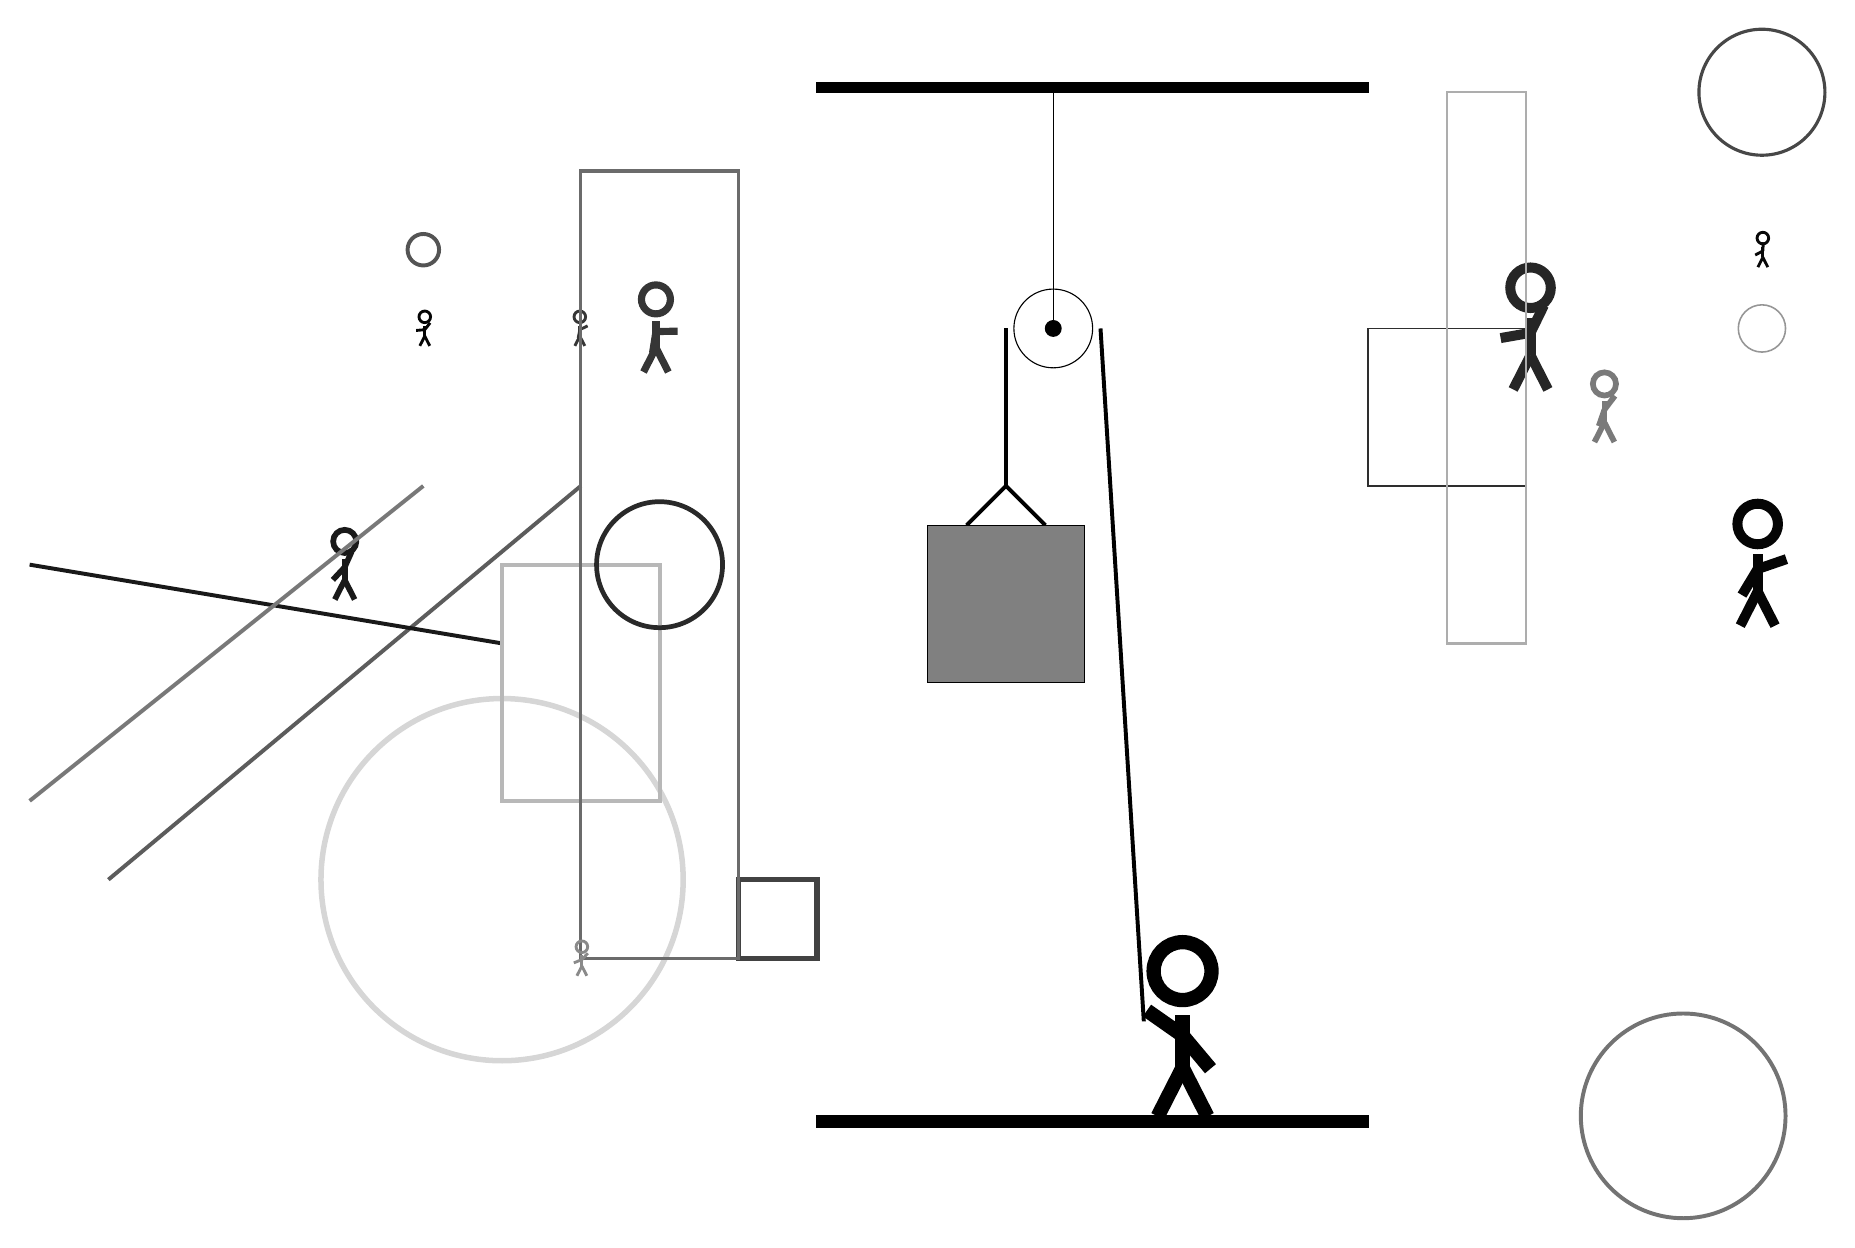
\begin{tikzpicture}
		%%%%% START %%%%%
		
		\draw[fill=black] (-2, 10) rectangle (5, 10.125);
		
		\draw (1, 7) circle (0.5);
		\draw[fill=black] (1, 7) circle (0.1);
		\draw (1, 10) -- (1, 7);
		
		\draw[line width=0.5mm] (-0.1, 4.5) -- (0.4, 5.0) -- (0.9, 4.5);
		\draw[fill=black!50] (-0.6, 4.5) rectangle (1.4, 2.5);
		
		\node[line width=0.6mm, color=black!79] at (-5, 7) {\Strichmaxerl[2][79][26]};
		
		\draw[line width=0.5mm, color=black!64](-5, 5) -- (-11, 0);
		\draw[line width=0.5mm, color=black!90](-6, 3) -- (-12, 4);
		\draw[line width=0.7mm, color=black!74] (-2, 0) rectangle (-3, -1);
		
		\draw [line width=0.5mm, color=black!19](-7, 7) circle (0.0);
		\draw [line width=0.7mm, color=black!16](-6, 0) circle (2.3);
		\draw[line width=0.5mm, color=black!28] (-4, 1) rectangle (-6, 4);
		
		\draw [line width=0.5mm, color=black!55](9, -3) circle (1.3);
		\draw[line width=0.4mm, color=black!58] (-3, -1) rectangle (-5, 9);
		\draw [line width=0.4mm, color=black!72](10, 10) circle (0.8);
		\node[line width=0.6mm, color=black!46] at (-5, -1) {\Strichmaxerl[2][22][47]};
		\draw[line width=0.2mm, color=black!82] (7, 5) rectangle (5, 7);
		\draw [line width=0.2mm, color=black!41](10, 7) circle (0.3);
		\node[line width=0.7mm, color=black!98] at (10, 4) {\Strichmaxerl[7][59][19]};
		\draw [line width=0.6mm, color=black!84](-4, 4) circle (0.8);
		\node[line width=0.4mm, color=black!98] at (-7, 7) {\Strichmaxerl[2][5][52]};
		
		\node[line width=0.3mm, color=black!85] at (7, 7) {\Strichmaxerl[7][10][64]};
		\node[line width=0.3mm, color=black!90] at (-8, 4) {\Strichmaxerl[4][47][66]};
		\draw[line width=0.3mm, color=black!32] (7, 10) rectangle (6, 3);
		\node[line width=0.7mm, color=black!97] at (10, 8) {\Strichmaxerl[2][28][87]};
		\draw [line width=0.5mm, color=black!67](-7, 8) circle (0.2);
		
		\node[line width=0.6mm, color=black!52] at (8, 6) {\Strichmaxerl[4][71][53]};
		
		\draw[line width=0.5mm, color=black!53](-7, 5) -- (-12, 1);
		\node[line width=0.5mm, color=black!79] at (-4, 7) {\Strichmaxerl[5][81][1]};
		
		\draw[line width=0.5mm] (0.4, 7) -- (0.4, 5.0);
		\centerarc[line width=0.5mm](1, 7)(0:180:0.6);
		\draw[line width=0.5mm](1.6, 7) -- (2.15, -1.8);
		
		\node at (2.6, -1.9) {\Strichmaxerl[10][-35][-50]};
		
		\draw[fill=black] (-2, -3) rectangle (5, -3.15);
		
		%%%%% END %%%%%
	\end{tikzpicture}
\end{document}